%%%%%%%%%%%%%%%%%%%%%%%%%%%%%%%%%%%%%%%%%
% Beamer Presentation
% LaTeX Template
% Version 1.0 (10/11/12)
%
% This template has been downloaded from:
% http://www.LaTeXTemplates.com
%
% License:
% CC BY-NC-SA 3.0 (http://creativecommons.org/licenses/by-nc-sa/3.0/)
%
%%%%%%%%%%%%%%%%%%%%%%%%%%%%%%%%%%%%%%%%%

%----------------------------------------------------------------------------------------
%	PACKAGES AND THEMES
%----------------------------------------------------------------------------------------

\documentclass{beamer}

\mode<presentation> {

% The Beamer class comes with a number of default slide themes
% which change the colors and layouts of slides. Below this is a list
% of all the themes, uncomment each in turn to see what they look like.

\usetheme{default}
%\usetheme{AnnArbor}
%\usetheme{Antibes}
%\usetheme{Bergen}
%\usetheme{Berkeley}
%\usetheme{Berlin}
%\usetheme{Boadilla}
%\usetheme{CambridgeUS}
%\usetheme{Copenhagen}
%\usetheme{Darmstadt}
%\usetheme{Dresden}
%\usetheme{Frankfurt}
%\usetheme{Goettingen}
%\usetheme{Hannover}
%\usetheme{Ilmenau}
%\usetheme{JuanLesPins}
%\usetheme{Luebeck}
%\usetheme{Madrid}
%\usetheme{Malmoe}
%\usetheme{Marburg}
%\usetheme{Montpellier}
%\usetheme{PaloAlto}
%\usetheme{Pittsburgh}
%\usetheme{Rochester}
%\usetheme{Singapore}
%\usetheme{Szeged}
%\usetheme{Warsaw}

% As well as themes, the Beamer class has a number of color themes
% for any slide theme. Uncomment each of these in turn to see how it
% changes the colors of your current slide theme.

%\usecolortheme{albatross}
%\usecolortheme{beaver}
%\usecolortheme{beetle}
%\usecolortheme{crane}
%\usecolortheme{dolphin}
%\usecolortheme{dove}
%\usecolortheme{fly}
%\usecolortheme{lily}
%\usecolortheme{orchid}
%\usecolortheme{rose}
%\usecolortheme{seagull}
%\usecolortheme{seahorse}
%\usecolortheme{whale}
%\usecolortheme{wolverine}

%\setbeamertemplate{footline} % To remove the footer line in all slides uncomment this line
%\setbeamertemplate{footline}[page number] % To replace the footer line in all slides with a simple slide count uncomment this line

%\setbeamertemplate{navigation symbols}{} % To remove the navigation symbols from the bottom of all slides uncomment this line
}

\usepackage{graphicx} % Allows including images
\usepackage{booktabs} % Allows the use of \toprule, \midrule and \bottomrule in tables
\usepackage{tikz}

%----------------------------------------------------------------------------------------
%	TITLE PAGE
%----------------------------------------------------------------------------------------

\title[Short title]{Spectral Image Analysis for \\Medical Imaging} % The short title appears at the bottom of every slide, the full title is only on the title page

\author{Michael Painter} % Your name
\institute[UoC] % Your institution as it will appear on the bottom of every slide, may be shorthand to save space
{
University of Cambridge \\ % Your institution for the title page
\medskip
\textit{mp703@cam.ac.uk} % Your email address
}
\date{4th February 2016} % Date, can be changed to a custom date

\begin{document}

\begin{frame}
    \titlepage % Print the title page as the first slide
\end{frame}

%----------------------------------------------------------------------------------------
%	PRESENTATION SLIDES
%----------------------------------------------------------------------------------------

\begin{frame}
    \frametitle{Overview of Project - What am I doing?}

    \begin{itemize}
        \item Investigating use of \textit{spectral images} to help with medical diagnosis.
        \item So we now consider a \textit{data cube} $I(x,y,\lambda)$. (E.g. $\lambda \in \{R, G, B\}$).
        \item The goal is to use the additional spectral information to help perform image segmentation.
        \item This is useful in medical imaging as a tool for diagnosis.
        \item We will use machine learning, specifically we will use Neural Nets and Random Forests.
        \item To be useful we will also need to deal with noisy data.
    \end{itemize}
\end{frame}

%------------------------------------------------


\begin{frame}
    \frametitle{Random Forests}
    \begin{block}{}
        \begin{figure}[H]
            \centering

            \tikzset{QuestionNode/.style = { rectangle, rounded corners, shade, 
                          top color = white, bottom color = blue!50!black!20, 
                          draw = blue!40!black!60, very thick, text ragged },
                      EdgeNodeStyle/.style = {draw = none}, above,
                      EmptyNode/.style = {draw = none}}
            \begin{tikzpicture}
                [
                    sibling distance = 3cm,
                    level distance = 4cm,
                    edge from parent/.style = {draw, arrows = ->},
                    level 1/.style = {sibling distance = 3cm, level distance = 3cm},
                    level 2/.style = {sibling distance = 1.5cm, level distance = 3cm},
                ]
                \node [QuestionNode] {Blond hair?}
                    child {
                        node [QuestionNode] {Brown hair?}
                        child {
                            node [EmptyNode] {$\vdots$}
                            edge from parent
                              node [EdgeNodeStyle, left] {no}
                        }
                        child {
                            node [EmptyNode] {$\vdots$}
                            edge from parent
                              node [EdgeNodeStyle, right] {yes}
                        }
                        edge from parent node [EdgeNodeStyle, left] {no}
                    }   
                    child {
                        node [QuestionNode] {Blue eyes?}
                        child {
                            node [EmptyNode] {$\vdots$}
                            edge from parent
                              node [EdgeNodeStyle, left] {no}
                        }
                        child {
                            node [EmptyNode] {$\vdots$}
                            edge from parent
                              node [EdgeNodeStyle, right] {yes}
                        }
                        edge from parent node [EdgeNodeStyle, right] {yes}
                    };
            \end{tikzpicture}

            \caption{Example of (part of) a tree used to classify humans.}
        \end{figure}
    \end{block}
\end{frame}

\begin{frame}
    \frametitle{Random Forests}

    \begin{block}{}
        \begin{itemize}
            \item Forest = set of trees.
            \item Trees `vote' towards a winning class.
        \end{itemize}

        \begin{figure}[H]
            \centering
            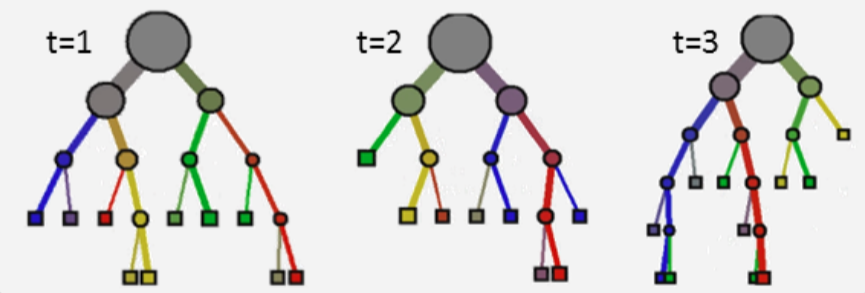
\includegraphics[scale=0.25]{Forests.png}
            \caption{\cite{r1}}
        \end{figure}
    \end{block}
\end{frame}

\begin{frame}
    \frametitle{Random Forests}

    \begin{block}{}
        \begin{itemize}
            \item Use \textit{weak learners} to split the training sequence up.
            \item Want the split that leads to the optimal \textit{information gain}.
            \item Can't possibly try every way of splitting, so search a random subspace.
        \end{itemize}

        \begin{figure}[H]
            \centering
            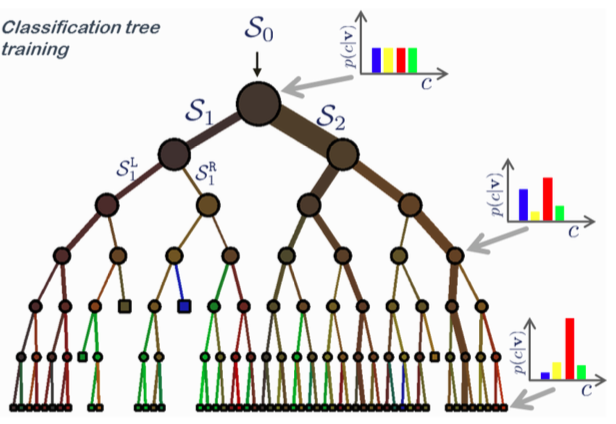
\includegraphics[scale=0.25]{ProbabilityTree.png}
            \caption{\cite{r1}}
        \end{figure}
    \end{block}
\end{frame}

\begin{frame}
    \frametitle{Progress - Schedule}

    \begin{block}{Completed Work}
        The project is on schedule as I have implemented the following:
        \begin{itemize}
            \item Random forests library.
            \item `DataCube' interface.
            \item Pixel labelling using random forests.
            \item Pixel labelling using Encog. (A machine learning library in Java with Neural Nets).
        \end{itemize}
    \end{block}


    \begin{block}{Work remaining}
        \begin{itemize}
            \item De noising images with Poisson noise.
            \item Get it working on some real images.
            \item Compare the implementations on how they perform (speed and accuracy).
        \end{itemize}
    \end{block}
\end{frame}

\begin{frame}
    \frametitle{Progress - Schedule}

    \begin{block}{Difficulties}
        \begin{itemize}
            \item Some data captured by separate devices, so need to be aligned.
            \item Lack of training data in some cases, but may be able to generate some.
        \end{itemize}
    \end{block}
\end{frame}

\begin{frame}
    \frametitle{Progress - Example}

    \begin{figure}[H]
        \centering
        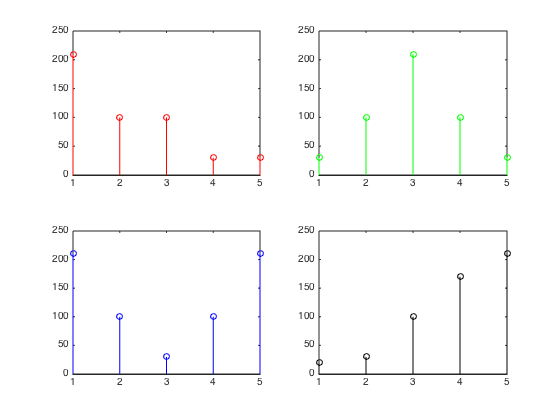
\includegraphics[scale=0.3]{toyImageProfiles.png}
    \end{figure}

    \begin{columns}[c]
        \column{.47\textwidth} % Left column and width
        
\includegraphics[scale=0.15]{Interpolated5DimImage1.png} \hspace{0.3pt}
        
\includegraphics[scale=0.15]{Interpolated5DimImage2.png} \hspace{0.3pt}
        
\includegraphics[scale=0.15]{Interpolated5DimImage3.png} \\ \hspace{17pt}
        
\includegraphics[scale=0.15]{Interpolated5DimImage4.png} \hspace{0.3pt}
        
\includegraphics[scale=0.15]{Interpolated5DimImage5.png}

        \column{.08\textwidth}
        $\rightarrow$

        \column{.45\textwidth}
        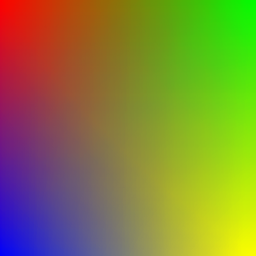
\includegraphics[scale=0.2]{rf.png} \hspace{0.3pt}
        
\includegraphics[scale=0.2]{rf256.png} \\
        
\includegraphics[scale=0.2]{rf1000.png} \hspace{0.3pt}
        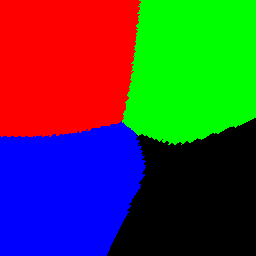
\includegraphics[scale=0.2]{nn.png}
    \end{columns}
\end{frame}

\begin{frame}
    \frametitle{Real Images}
        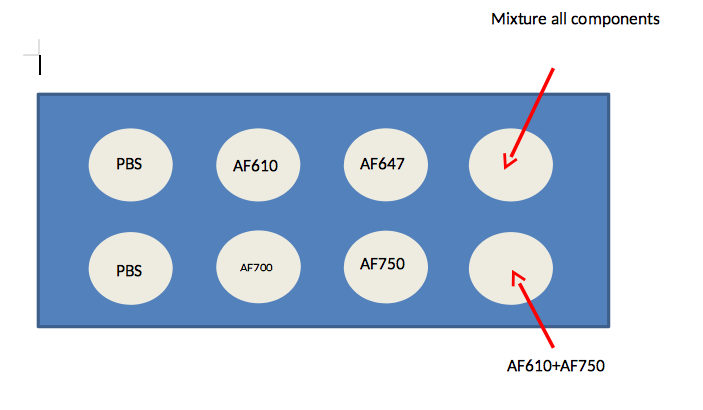
\includegraphics[scale=0.2]{wells.png}
        \vspace{1mm}
        
\includegraphics[scale=0.1]{wavelet_den_45.png}

        \vspace{1mm}
        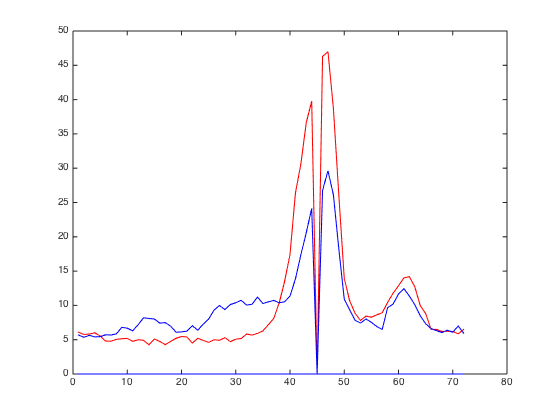
\includegraphics[scale=0.25]{contrastAgentResponses1.png} 

\end{frame}


\begin{frame}
    \frametitle{References}
    \footnotesize{
        \begin{thebibliography}{99} % Beamer does not support BibTeX so references must be inserted manually as below
            \bibitem[Chriminisi, Shotton, Konukoglu, 2012]{r1} Antonio Criminisi, Jamie Shotton, and Ender Konukoglu (2012)
            \newblock Decision Forests: A Unified Framework for Classification, Regression, Density Estimation, Manifold Learning and Semi-Supervised Learning
            \newblock \emph{Foundations and Trends® in Computer Graphics and Vision} 7(2-3), 81 -- 227.
        \end{thebibliography}
    }
\end{frame}

\end{document} 